\documentclass[a4paper,oneside,12 pt]{article}
\usepackage[french]{babel}
\usepackage[T1]{fontenc}
\usepackage{verbatim}
\usepackage[utf8]{inputenc}
\usepackage{multirow}
\usepackage{graphicx}
\title{Documentation des actions }
\begin{document}
\maketitle

\section{Peuplement et environnement}
Dans cette simulation, un seul peuplement Civ1 avec une centaine d'agents.

Ceux-ci, ont intialement tous les mêmes caractéritisques : sommeil (50) et vie (20).

La simulation aura lieu dans un environnement constitués de patches de deux types de  terrains : forêt et prairie de \textit{passability} 25 et 35.

Après chargement de l'environnement Test.metaciv, on dispose de l'environnement et de la localisation de départ de Civ1 (cf. Figure \ref{loca})
\begin{figure}[!ht]
\begin{center}
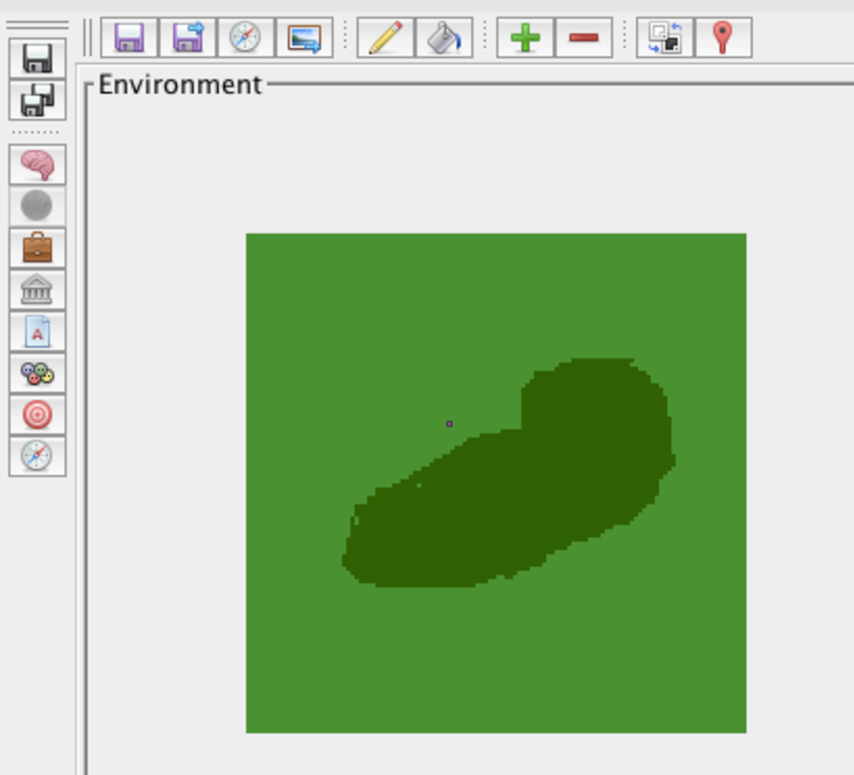
\includegraphics[scale=0.5]{locas1.pdf}
\caption[loca]{Environnement \\}
\label{loca}
\end{center}
\end{figure} 

L'inventaire des agents pourrait potentiellement comporter les objets Baton, Céréale, Outil.

Céréale a l'effet possession qui ajoutera 0.2 au poids du cogniton Produireautrechose à chaque foisqu'un agent ajoutera un objet céréale à son inventaire.

En ce qui concerne les aménagements \textit{(facility)}, on trouve Champ et Maison.
Champ a un effet permanent Renforcer agriculture qui ajoute  0.05 au poids du cogniton Agriculteur à chaque fois qu'il utilise le champ.

Maison a un effet permanent Dormir qui ajoute 40.0 à l'attribut Sommeil de l'agent à chaque fois qu'il utilise cet aménagement.

\section{Cogniton, Plan, Actions}



\begin{figure}[!ht]
\begin{center}
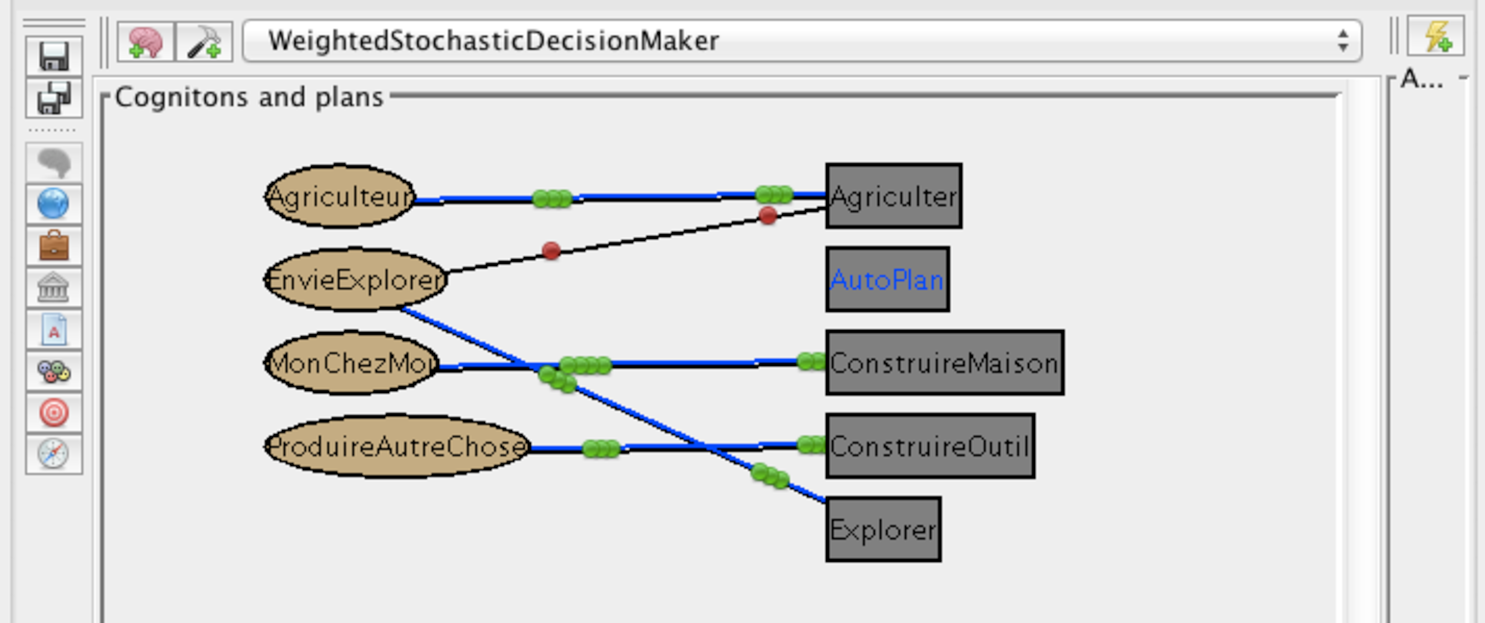
\includegraphics[scale=0.5]{CogPl.pdf}
\caption[CP]{Environnement \\}
\label{CP}
\end{center}
\end{figure} 

La figure \ref{CP}) présente la \textit{cognition} : l'ensemble des cognitons (Agriculteur, EnvieExplorer, MonChezMoi, ProduireAutreChose) et plans (Autoplan et Agriculter, ConstruireMaison, ConstruireOutil, Explorer) ainsi que les liens conditionnels (bleu) et d'influence (noir).

Les billes verte correspondent à une influence positive, les rouge à une influence négative et leur quantité dénonce le poids.

Par exemple, Agriculter est lié conditionnellement au cogniton Agriculteur (qui influence aussi positivement ce plan) ; par contre  le cogniton EnvieExplorer influence négativement ce même plan.

Un clic droit sur chaque cogniton donne le détail sur celui-ci (nom, type et pourcentage d'agent qui auront     ce cogniton à leur création) et sur les liens le concernant.

\textit{Remarque : le dosage du pourcentage est important dans le modèle et pour la simulation}

// à détiller

Pour accéder à la description des actions d'un plan (clic gauche), si les actions L double clicquer sur elles jusqu'à déploiement complet des actions du plan.


Autoplan
	2 actions A\_ChangeAttribute (portant sur sommeil et vie)
	
	
Plan ConstruireMaison

L'arbre des actions déployé est représenté sur la figure \ref{PL}.
\begin{figure}[!ht]
\begin{center}
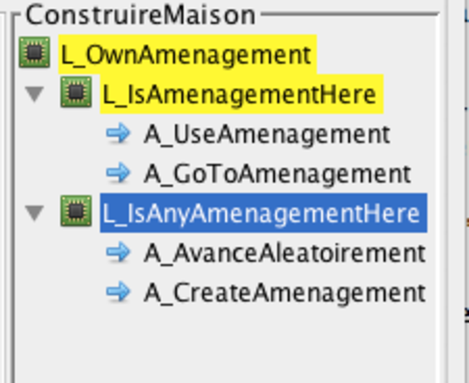
\includegraphics[scale=0.5]{planex.pdf}
\caption[PL]{Arbre des actions du plan ConstruireMaison \\}
\label{PL}
\end{center}
\end{figure} 

SI j'ai une maison (n'importe où) ALORS
		\textit{action interne 1 niveau 1}
		SI j'ai une maison sur le patch où je suis ALORS
				\textit{action interne1 niveau 2 }
				j'utilise cette maison (et par suite je gagne 40 de sommeil)
		SINON
				\textit{action interne2 niveau 2 }
				je me déplace vers le patch de ma maison la plus proche;

SINON
		\textit{action interne2 niveau 2 }
		SI sur le patch où je suis, existe un quelconque aménagement ALORS
			\textit{ action interne 1 niveau 2} 
			 j'avance aléatoirement d'un pas (le patch étant occupé)
		SINON
			\textit{action interne 2 niveau 2 }
			je crée une maison sur le patch 
;


\end{document}

